% Resolving conflicts with vector clocks

% The original Dynamo, like the open-source Voldemort and Riak, was a key/value database. Thus, objects would need to be serialized in a format such as json. For example, I might have a user object with key jbellis and value of {'email': 'jbellis@example.com', 'phone': '555-5555'}. We'll call this initial value V0.

% Next, suppose we update the email address, changing the value to V1 of {'email': 'jbellis@illustration.com', 'phone': '555-5555'}. Some failure causes this to only be written to one replica. Later, we update the phone number, but we read from a different replica so we start from the original value V0 (with the original email address), so we write V2 {'email': 'jbellis@example.com', 'phone': '444-4444'}.

% (Note that failure -- whether actual machine failure, network failure, or even load shedding -- can cause "conflicting" updates even with a single client and no concurrency.)

% Since our object values are opaque blobs to this system, a naive last-write-wins conflict resolution policy will result in discarding the V1 email address change in favor of the V2 phone number update. This is why it's so easy to lose data using last-write-wins conflict resolution in a key/value system like Riak.

% Vector clocks solve this problem by allowing the database to push conflict resolution back out to the client. Skipping a lot of details, the database would retain both V1 and V2, and when a client next reads key jbellis, it would return both versions and tell the client, "you figure out what you want the value to be now." The client can then deserialize the objects and merge the separately updated fields without data loss to the intended value of {'email': 'jbellis@illustration.com', 'phone': '444-4444'}.
% https://www.datastax.com/dev/blog/why-cassandra-doesnt-need-vector-clocks
%
% Footnotes
%
\def \naturalkey {Ein Schlüssel, der sich aus einem Attribut des Objekts ergibt oder sich aus mehreren Attributen zusammensetzt. So könnte ein sprechender Schlüssel von Jean-Luc Picard mit der E-Mail-Adresse picard@enterpise.com beispielsweise `picard@enterprise.com` (E-Mail) oder `Jean-LucPicard` (Zusammensetzung aus Vor- und Nachnamen) sein.}
\def \logicalclock {Eine Logische Uhr ist eine Komponente die dazu dient, dem Datenobjekt einen eindeutigen Zeitstempel zuzuweisen. Die bekanntesten Verfahren für Logische Uhren in verteilten Systemen sind die Lamport-Uhr und die Vektoruhr. Beide verwenden Zähler die sich bei jedem Ereignis erhöhen. Einfach gesagt besteht die Lamport-Uhr aus einem Zeitstempel und einem Zähler, die Vektoruhr aus einem Zeitstempel und einem Vektor -- einer Liste aus Zählern.}
%
%
\begin{description}[leftmargin=0.5cm,style=nextline]
  % ID
  \item[Methode ID0 -- UUID:]
    Zur Identifizierung eines Adressbucheintrags wird eine \gls{UUID} verwendet. Es wird sowohl auf dem Client als auch auf dem Server ein Kontakt mit dem Namen `Amilia Pond` erstellt.
    Währenddessen tritt Fall \it{b} oder \it{c} ein und beide Parteien können nicht miteinander kommunizieren. Nach der Synchronisation existieren zwei Kontakteinträge mit gleichem Namen, aber unterschiedlicher ID.
    Sie sind voneinander zu unterscheiden und können einzeln behandelt werden.\\
%
  \item[Methode ID1 -- sprechender Schlüssel:]
    Zur Identifizierung eines Adressbucheintrags wird ein sprechender Schlüssel\footnote{\naturalkey} verwendet.
    Sowohl auf dem Client als auch auf dem Server wird ein Kontakt mit dem Namen `Amilia Pond` und dem sprechenden Schlüssel `amiliapond` erstellt.
    Währenddessen tritt Fall \it{b} oder \it{c} ein.
    Es ist nicht zu ermitteln, ob derselbe Kontakt doppelt angelegt wurde, wenn beide Kontakteinträge sich unterscheiden, welcher der beiden korrekt ist oder ob es sich bei den Einträgen um zwei Personen mit demselben Namen handelt.\\
  %
  %
  % Version
  \item[Methode V0 -- Versionsnummer:]
    Zur Versionierung eines Adressbucheintrags werden Versionsnummern verwendet. Der Kontakt `Amilia` hat die Version `1.0.0`.
    Sowohl auf dem Client, als auch auf dem Server wird der Kontakt bearbeitet und aktualisiert und beide geben ihm die Versonsnummer `2.0.0`.
    Währenddessen tritt Fall \it{b} oder \it{c} ein und beide Parteien können nicht miteinander kommunizieren.
    Bei der Synchronisation entsteht ein Konflikt weil es zwei unterschiedliche Einträge mit derselben Verion gibt.\\
  %
  % Zeitstempel
  \item[Methode V1 -- Zeitstempel:]
    Zur Versionierung eines Adressbucheintrags wird ein Zeitstempel verwendet. Der Kontakt `Amilia` hat die initiale Version `2018-04-03 10:00:00Z`.
    Amilia ist umgezogen und ihre Adresse ändert sich. Der Eintrag wird bearbeitet und hat nun die Version `2018-04-13 11:44:22Z`.
    Während der Editierung tritt Fall \it{b} oder \it{c} ein.
    Es stellt sich heraus, dass die Hausnummer einen Zahlendreher hat und es wird sofort, immer noch offline, berichtigt. `Amilia` hat nun die Version `2018-04-13 11:45:33Z`.\\
    Der Server hat eine eigene Uhr mit spätere Uhrzeit als der Client.
    So hat nach der Synchronisation der später korrigierte Eintrag einen früheren Zeitstempel.
    Es wird die falsche, alte Adresse gespeichert, die korrekte hat den älteren Zeitstempel und wird verworfen.\\
    Diese Variante funktioniert in vielen Fällen gut. Trotzdem kommt es selbst in großen Firmen wie z.B. Google zu Problemen\footnote{\url{https://support.google.com/accounts/answer/185834?hl=en\#sync}}, wenn verschiedene Geräte eine eigene Uhr besitzen.\\
    Des Weiteren gibt es die Möglichkeit, dass auf dem einen Gerät die Hausnummer berichtigt wurde und auf einem anderen, zur ungefähr selben Zeit, ein Zusatz zur Adresse gespeichert wird. Das könnte die Etage sein in der Amilia wohnt. Dann gibt es zwei Versionen mit unterschiedlichen Zeitstempeln und eine davon wird in jedem Fall verworfen. Auch wenn beide Versionen richtig sind.\\
  %
  % Logische Uhr
  \item[Methode V2 -- Logische Uhr:]
    Weil der Zeitstempel so fehleranfällig ist, wurde die Logische Uhr zur Versionierung von Objekten in Verteilten Systemen entwickelt.\\
    Zur Versionierung eines Adressbucheintrags wird eine Logische Uhr\footnote{\logicalclock} verwendet.
    Der Kontakt `Amilia` hat die Version \todo{Beispiel Logische Uhr?}.
    Amilias Adresse ändert sich und wird auf dem Client angepasst.
    Währenddessen tritt Fall \it{b} oder \it{c} ein.
    Amilia sieht ihre falsche Hausnummer und berichtigt diese ebenfalls.
    Bei der Synchronisation kommt es zum Konflikt. \todo{wirklich? auch wenn das Ergebnis dasselbe ist?}\\
    %
    % Hash
    % hash: { name: Amilia Pond, phone: 0152397645, email: Amilia@pond.com }
  \item[Methode V3 -- Inhaltsbasierte Version:]% CAV fail
    Zur Versionierung eines Adressbucheintrags wird eine inhaltsbasierte Version verwendet. Um eine Zuordnung zwischen Inhalt und Version machen zu können kommen \Gls{Hash}funktionen zum Einsatz. Hierbei wird als Version der Hashwert des Adressbucheintrags gespeichert.\\
    Dem Kontakt `Amilia` ist die Version `5560348cec1b08c3d53e1508b4a46868` zugeordnet. Amilias Telefonnummer ändert sich und wird auf dem Client angepasst, während dieser offline ist.
    Im selben Status berichtigt der Client die Telefonnummer. Bei der Synchronisation kommt es zum Konflikt, da es nun zwei Einträge mit unterschiedlichem Inhalt, aber identischer Version gibt und nicht festzustellen ist, welche Version die neuere ist.\\
    %
    % Hash Liste
  \item[Methode V4 -- Liste von inhaltsbasierten Versionen:]
    Zur Versionierung eines Adressbucheintrags wird eine geordnete Liste von inhaltsbasierten Versionen verwendet.
    Dem Kontakt `Amilia` ist eine Liste von Versionen mit einem Eintrag `5560348cec1b08c3d53e1508b4a46868` zugeordnet.
    Amilias Telefonnummer ändert sich und wird auf dem Client angepasst, während dieser offline ist. Im selben Status berichtigt der Client die Telefonnummer.
    Jede Aktion fügt der Versionsliste einen neuen Hashwert hinzu.
    Auch wenn der Content des Adressbucheintrags in den zwei letzten Versionen identisch ist, kann festgestellt werden welcher der neueste Eintrag ist.
    Bei der Synchronisation kommt es zum Konflikt weil der Kontakt Amilia mit unteschiedlichen Informationen existiert.\\
    Beide konfliktbehafteten Versionen werden verschachtelt in der Liste gespeichert.
    In diesem Fall sieht die Liste so aus: \\
    '[[ 88da3f8d82ab58551d2a48d74d9a4986, 5560348cec1b08c3d53e1508b4a46868 ], 88da3f8d82ab58551d2a48d74d9a4986 ]' -- eine Liste der beiden konfliktbehafteten Versionen am Anfang der Liste.
\end{description}
% \begin{figure}[H]
%   \centering
%   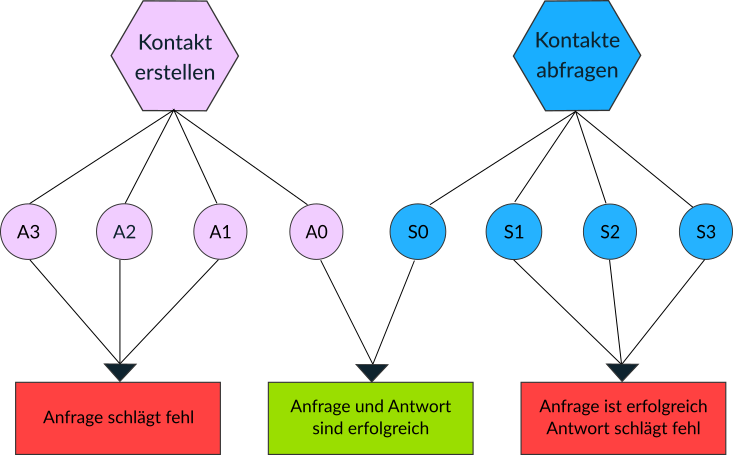
\includegraphics[width=0.8\textwidth]{Szenarien}
%   \grayRule
%   \caption[Szenarien]{Szenarien und Fälle}
%   \label{fig:scenarios}
% \end{figure}
%
% ERGEBNIS
%
\subsubsection*{Ergebnis}
Die Methoden \it{ID0} und \it{ID1} beschreiben die Identifizierung einzelner Kontakte. Eine eindeutige Identifizierung des Kontakts ist im Methode \it{ID0}, mittels der Verwendung einer \gls{UUID}, gewährleistet.
% Die Szenarien \it{V1}, \it{V2} und \it{V4}, \it{V5} beschreiben Situationen mit demselben Ausgangspunkt. In einem Fall kommt zu keinem Konflikt, in dem nächsten schon. Deswegen können \it{V1} und \it{V2}, sowie \it{V4} und \it{V5} zusammengefasst werden.
Es wird deutlich, dass es in jedem Fall zu einem Konflikt kommen kann. Es gilt zu unterscheiden in welchen Fällen mit Konflikten umgegangen werden muss weil sonst Daten verloren gehen.